\section{Publish/Subscribe-Systeme}
\label{chap:grundlagen:pubsub}
\missing{schöner: Zur Verteilung von Events (Event-Dissemination) gibt es vielfältige Systeme, wie MessagePassing .. many faces!}

Publish/Subscribe-Systeme sind Forschungszweck vieler wissenschaftlicher Arbeiten (z.B. \cite{Banerjee2001Comparative, Liu2003Survey, Muhl2002LargeScale, FiegeSecurity, Castro2002Scribe}) und daher gut erforscht und beschrieben. Diese Systeme eigenen sich auf Grund ihres Aufbaus sehr gut zur Eventverteilung in dezentralen Systemen, da sie gegenüber anderen Nachrichtensystemen (wie z.B. \emph{message passing} oder \emph{rpc}) in drei orthogonalen Dimensionen\index{Publish/Subscribe!orthogonale Dimensionen} skalieren \cite{PatrickTh2003Many}.

\begin{figure}[htbp]
\centering
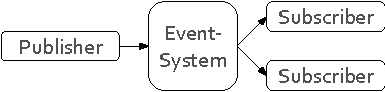
\includegraphics{grafics/pubsub_black_box.pdf}
\caption{Schema eines Publish/Subscribe-Systemes.}
\label{fig:pubsub_black_box}
\end{figure}

\paragraph{räumliche Trennung}
Wie in \Fref{fig:pubsub_black_box} zu sehen ist, trennt das Event-System Publisher und Subscriber räumlich voneinander. Diese Trennung bezieht sich nicht alleine auf verschiedene Schichten einer eine Applikation, sondern kann auch über Applikationsgrenzen oder gar Rechnergrenzen gehen.\\
Weiterhin skaliert ein solches System besser, da der Publisher nur mit dem Event-System kommuniziert und dieses darauf ausgelegt ist, viele Subscribern zu bedienen.

\cite{PiEyKoSh2007-PubSubAPI} gibt einen Vorschlag für eine generische API\index{Publish/Subscribe!generische API} für Publish/Subscribe-Systeme und unterteilt die Kompabilität verschiedener Systeme in drei Level. Das höchste Level beschreibt einen Datenaustausch der an XML-RPC angelegt ist. Implementieren Systeme dieses Level, so können verschiedene Publish/Subscribe-Systeme miteinander kommunizieren.

\paragraph{zeitliche Trennung}
Publisher und Subscriber sind in ihren Aktionen mit dem Event-System zeitlich getrennt. Ein Publisher muss kein Wissen über Subscriber haben und umgekehrt. Dies bedeutet dass sich ein Subscriber am System anmelden kann, obwohl kein Publisher vorhanden ist. Für Publisher gilt dies analog. Bei \emph{message-passing} ist dies nicht möglich, da die Gegenseite bekannt sein muss.

\paragraph{asynchrone Verarbeitung}
Das Senden einer Nachricht ist für den Publisher nicht blockierend. Die Auslieferung der Nachricht erfolgt für die Subscriber ebenfalls nicht blockierend, da ihnen die Nachricht per Callback zugestellt wird und damit die Verarbeitung vom Event-System aus gestartet wird.


\subsection{Arten von Publish/Subscribe-Systemen}
Publish/Subscribe-Systeme gibt es grundsätzlich in zwei Ausführungen:
\begin{itemize}
\item kanalbasiert (\emph{topic-based})
\item filterbasiert (\emph{content-based})
\end{itemize}

Beide Varianten haben Vor- und Nachteile, die 

\subsubsection{Kanalbasiert}
\label{chap:grundlagen:pubsub:kanalbasiert}
Nachrichten in kanalbasierten\index{Publish/Subscribe!kanalbasiert} Systemem werden im Kontext von Kanälen oder Topics behandelt. Nachrichten können, nur in Verbindung mit einem Topic an das System übergeben werden. Clients können sich für verschiedene Kanäle einschreiben und erhalten nur diese Nachrichten.
\missing{Das ist nicht schön beschrieben!}

Listing \vref{code:pubsub-topicbased} zeigt die mögliche API eines solchen Systemes, diese variiert aber von System zu System. Jedoch ist klar ersichtlich, dass die API stark vom Kanalnamen geprägt ist. \emph{deliver\_callback} bezeichnet hier eine Funktion, die das System bei neuen Nachrichten aufrufen soll.

\lstinputlisting[caption={Exemplarische API eines topic-based Event-Systems}, label=code:pubsub-topicbased]{listings/pubsub_topicbased.cpp}

Kanalbasierte Systeme können sehr gut optimiert werden, da die Anzahl der Kanäle und deren Art zur Erstellungszeit meist bekannt ist. Selbst wenn zur Laufzeit neue Kanäle hinzugefügt werden, geschieht dies ebenfalls strukturiert und dient der internen Optimierung des Systems. Durch die Gruppierung der Nachrichten, müssen insgesamt weniger Nachrichten verschickt werden.

Filterungen sind in diesem Systemen meist nur clientseitig effizient möglich. Clients können die empfangenen Nachrichten filtern und unpassende Nachrichten verwerfen. Wird eine Filterung durch strukturierte Kanalnamen, wie z.B. \emph{TEAMSPEAK.TEAM\_EAGLE} oder \emph{TEAMSPEAK.TEAM\_RED}, ermöglicht, kann die Anzahl der zu versendenden Nachrichten reduziert wreden. Möchte ein Client alle \emph{TEAMSPEAK}-Nachrichten empfangen, muss für jeden Kanal eine eigene Subscribtion am System erfolgen.

Um das System im Vorraus filtern zu lassen, müsste ein geeigneter Filter bei der Anmeldung übergeben werden. Damit das Event-System die Nachrichten filter kann, müssen diese in einem vom System lesbaren Format vorliegen. Dies bedeutet, dass das Event-System und die Clients stärker gekoppelt sind oder dass durch selbstbeschreibende Nachrichtenformate die Nachrichtengröße aufgebläht wird.\\
\cite{PiEyKoSh2007-PubSubAPI} zeigt mit einem System aus XML basierten Nachrichten und XPath Filter das dies möglich ist. Weiterhin verbessert dies, wie oben angesprochen, die Interopabilität verschiedener Systeme.

Können keine selbstbeschreibende Nachrichtenformate genutzt werden, so müssen dem Event-System Callbacks zur Filterung zur Verfügung stehen. Diese Callback können jedoch erst auf Clientseite ausgeführt werden, was einen Transport der Nachricht zum Client bedingt. Dies widerspricht jedoch der Idee der Nachrichtenvermeidung durch Filterung. In \Fref{chap:konzeption_pubsub} wird beschrieben, wie solch eine Filterung jedoch auch gewinnbringend eingesetzt werden kann.

Ein prominenter Vertreter dieser Art ist Scribe \cite{Castro2002Scribe}, dessen Funktionsweise in \Fref{chap:related:scribe} genau beschrieben wird.

\subsubsection{Filterbasiert}
\label{chap:grundlagen:pubsub:filterbased}
In filterbasierten\index{Publish/Subscribe!filterbasiert} Systemen, gibt es streng genommen nur einen einzigen Kanal. Bei der Anmeldung muss der Client einen Filter übergeben. Das Event-System liefert nur die Nachrichten aus, die auf diesen Filter passen. Wie oben beschrieben, muss das Event-System zur Filterung die Nachrichten lesen können, bzw. müssen diese mit filterbaren Metadaten angereichert werden.\\
Listing \ref{code:pubsub-contentbased} zeit eine exemplarische API für solche Systeme. Statt eines Kanalnames wird bei der Subscription ein Filter übergeben. Über das zurückgegebene Handle kann sich ein Client wieder abmelden.

Filterbasierte Systeme sind nicht im gleichen Ausmaße optimierbar wie kanalbasierte Systeme, da jeder Client potentiell alle Nachrichten empfangen kann. Durch eine Anpassung der Filter sind diese Systeme jedoch flexibler in der Benutzung.

\lstinputlisting[caption={Exemplarische API eines content-based Event-Systems}, label=code:pubsub-contentbased]{listings/pubsub_contentbased.cpp}
